\documentclass[
11pt, % The default document font size, options: 10pt, 11pt, 12pt
codirector, % Uncomment to add a codirector to the title page
]{charter} 




% El títulos de la memoria, se usa en la carátula y se puede usar el cualquier lugar del documento con el comando \ttitle
\titulo{Sistema de Monitoreo Térmico de Bogies} 

% Nombre del posgrado, se usa en la carátula y se puede usar el cualquier lugar del documento con el comando \degreename
\posgrado{Carrera de Especialización en Sistemas Embebidos} 
%\posgrado{Carrera de Especialización en Internet de las Cosas} 
%\posgrado{Carrera de Especialización en Intelegencia Artificial}
%\posgrado{Maestría en Sistemas Embebidos} 
%\posgrado{Maestría en Internet de las cosas}

% Tu nombre, se puede usar el cualquier lugar del documento con el comando \authorname
\autor{Ing. Hernán Gomez Molino} 

% El nombre del director y co-director, se puede usar el cualquier lugar del documento con el comando \supname y \cosupname y \pertesupname y \pertecosupname
\director{Esp. Ing. Martín Harris}
\pertenenciaDirector{SOFSE - DNT} 
% FIXME:NO IMPLEMENTADO EL CODIRECTOR ni su pertenencia
\codirector{Ing. Guillermo Figini} % para que aparezca en la portada se debe descomentar la opción codirector en el documentclass
\pertenenciaCoDirector{SOFSE - DNT}

% Nombre del cliente, quien va a aprobar los resultados del proyecto, se puede usar con el comando \clientename y \empclientename
\cliente{Esp. Ing. Mariano Fernández Soler}
\empresaCliente{CENADIF}

% Nombre y pertenencia de los jurados, se pueden usar el cualquier lugar del documento con el comando \jurunoname, \jurdosname y \jurtresname y \perteunoname, \pertedosname y \pertetresname.
\juradoUno{Nombre y Apellido (1)}
\pertenenciaJurUno{pertenencia (1)} 
\juradoDos{Nombre y Apellido (2)}
\pertenenciaJurDos{pertenencia (2)}
\juradoTres{Nombre y Apellido (3)}
\pertenenciaJurTres{pertenencia (3)}
 
\fechaINICIO{24 de junio de 2021}		%Fecha de inicio de la cursada de GdP \fechaInicioName
\fechaFINALPlan{19 de agosto de 2021} 	%Fecha de final de cursada de GdP
\fechaFINALTrabajo{20 de junio de 2022}	%Fecha de defensa pública del trabajo final


\begin{document}

\maketitle
\thispagestyle{empty}
\pagebreak


\thispagestyle{empty}
{\setlength{\parskip}{0pt}
\tableofcontents{}
}
\pagebreak


\section*{Registros de cambios}
\label{sec:registro}


\begin{table}[ht]
\label{tab:registro}
\centering
\begin{tabularx}{\linewidth}{@{}|c|X|c|@{}}
\hline
\rowcolor[HTML]{C0C0C0} 
Revisión & \multicolumn{1}{c|}{\cellcolor[HTML]{C0C0C0}Detalles de los cambios realizados} & Fecha      \\ \hline
0      & Creación del documento.                                 &24/06/2021\\ \hline
1      & Se completa hasta el punto 5 inclusive.                 & 08/07/2021 \\ \hline
2      & Se cambio el título del documento.\newline
		 Se actualizó el punto 5. Supuestos del proyecto.\newline  
		 Se completa hasta el punto 9 inclusive.      		      & 15/07/2021 \\ \hline
3     & Se cambio cambió la designación de prioridades del punto 6.\newline 
		 Se completa hasta el punto 12 inclusive.      		      & 23/07/2021 \\ \hline
4     & Se actualizó el punto 5. Supuestos del proyecto.\newline 
		 Se completa la totalidad del documento.      		      & 03/08/2021 \\ \hline
\end{tabularx}
\end{table}

\pagebreak



\section*{Acta de constitución del proyecto}
\label{sec:acta}

\begin{flushright}
Buenos Aires, \fechaInicioName
\end{flushright}

\vspace{2cm}

Por medio de la presente se acuerda con el \authorname\hspace{1px} que su Trabajo Final de la \degreename\hspace{1px} se titulará ``\ttitle'', que consistirá esencialmente en la implementación del prototipo de un sistema que gestionará la información y alarmas de las temperaturas relevantes de los pares montados de la locomotora, y tendrá un presupuesto preliminar estimado de 600 hs de trabajo y \$ 1.272.152, con fecha de inicio \fechaInicioName\hspace{1px} y fecha de presentación pública \fechaFinalName.

Se adjunta a esta acta la planificación inicial.

\vfill

% Esta parte se construye sola con la información que hayan cargado en el preámbulo del documento y no debe modificarla
\begin{table}[ht]
\centering
\begin{tabular}{ccc}
\begin{tabular}[c]{@{}c@{}}Dr. Ing. Ariel Lutenberg \\ Director posgrado FIUBA\end{tabular} & \hspace{2cm} & \begin{tabular}[c]{@{}c@{}}\clientename \\ \empclientename \end{tabular} \vspace{2.5cm} \\ 
\multicolumn{3}{c}{\begin{tabular}[c]{@{}c@{}} \supname \\ Director del Trabajo Final\end{tabular}} \vspace{2.5cm} \\
%\begin{tabular}[c]{@{}c@{}}\jurunoname \\ Jurado del Trabajo Final\end{tabular}     &  & \begin{tabular}[c]{@{}c@{}}\jurdosname\\ Jurado del Trabajo Final\end{tabular}  \vspace{2.5cm}  \\
%\multicolumn{3}{c}{\begin{tabular}[c]{@{}c@{}} \jurtresname\\ Jurado del Trabajo Final\end{tabular}} \vspace{.5cm}                                                                     
\end{tabular}
\end{table}




\section{1. Descripción técnica-conceptual del proyecto a realizar}
\label{sec:descripcion}

%Objetivo del sistema original.
Las locomotoras CNR - CKD8, incorporadas a la flota de Trenes Argentinos, tienen integrado en su equipamiento original un sistema denominado Hot Box.

El objetivo principal del sistema es evitar la operación de la locomotora en una condición de sobretemperatura de rodamientos en los bogies (carros inferiores que contienen los ejes, sobre los que se soporta la carrocería) que pueda desencadenar en una falla catastrófica.

Para ello detecta la condición temprana de degradación mediante el monitoreo constante de la temperatura de operación en los puntos pasibles de falla.

%Descripción de sistema original.
El sistema está compuesto por:
\begin{itemize}
\item Dos cajas Hot Box ubicadas una en cada cabina de conducción, sobre el pupitre de mando. 
\item Un bus sensores con protocolo 1Wire.
\item 36 sensores de temperatura, ubicados 6 en cada par montado (conjunto de eje y ruedas).
\item Una conexión de comunicación entre ambas Hot Box.
\item Un conector frontal, ubicado en la Hot Box de la cabina 1, que permite la conexión de un sensor.
\end{itemize}
La disposición de estos componentes se muestra esquemáticamente en la figura 1.
\begin{figure}[h]
	\centering
	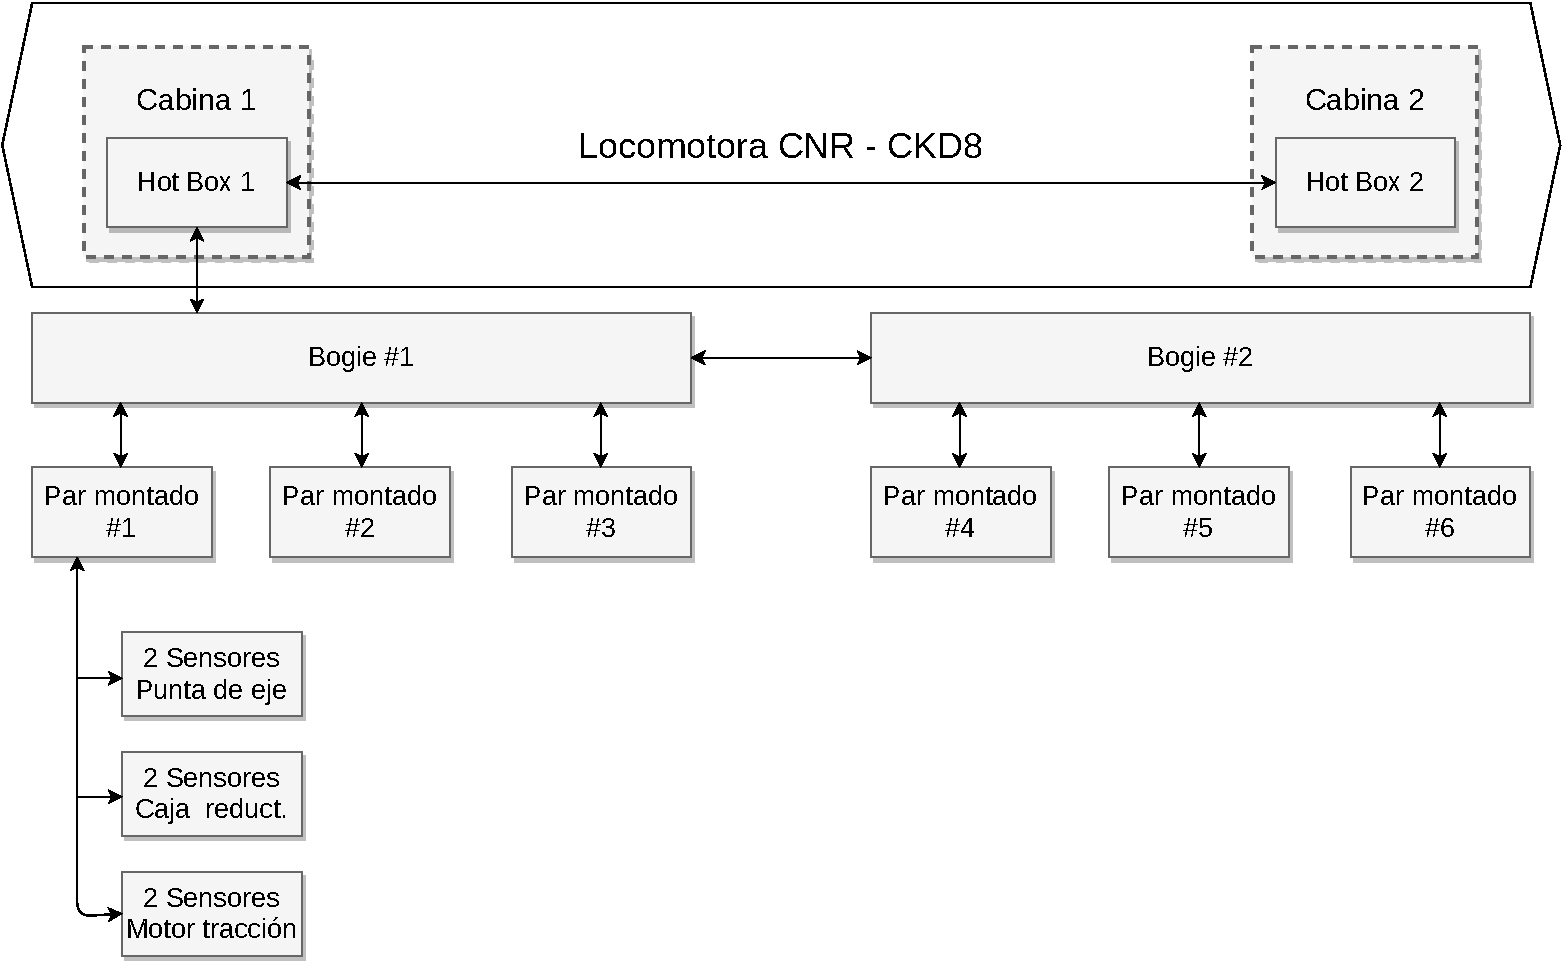
\includegraphics[angle=0,width=0.95\textwidth]{./Figuras/SMTB_bloques.pdf}
	\caption{Diagrama en bloques del sistema.}
	\label{fig:mesh1}
\end{figure}

Si bien las cajas presentan funcionalidades distintas, ambas integran un microcontrolador, 5 teclas idénticas y presentan la información al conductor mediante un display de 7 segmentos, de 6 dígitos, y una matriz de LEDs de 6 x 6.
Sus diferencias consisten en la conexión al bus y el conector frontal, que solo están implementados en la Hot Box 1.

%Problemas
El sistema original adolece de diversos problemas a la hora de realizar su mantenimiento:
\begin{itemize}
\item Diseño cerrado: la información puesta a disposición por el fabricante para la reparación de los componentes es inexistente en los manuales provistos. Los repuestos disponibles para adquisición en la fábrica solo contemplan el recambio de unidades completas.
\item Costos de reposición: los repuestos deben importarse del país de origen, lo que impacta fuertemente en los costos de adquisición. El fabricante es, además, el único proveedor del sistema a nivel global.
\item Soporte de postventa: el fabricante no provee la posibilidad de realizar cambios o mejoras al sistema. 
\end{itemize}

%Descripción del proyecto.
Con la motivación de corregir estos problemas, se propone desarrollar un reemplazo del sistema de diseño propio, con la máxima integración de componentes nacionales posible y reutilizando la instalación existente en las locomotoras. Adicionalmente, este desarrollo permitirá la nacionalización de las cadenas de valor que siempre resulta ventajosa para el país. 

Específicamente, el desarrollo comprenderá el reemplazo de ambas unidades Hot Box por las que se denominarán Unidad de Control e Interfaz (UCI) y los sensores de temperatura.
Las UCI conservarán el factor de forma original y su alimentación eléctrica de manera que el reemplazo de sistema solo implique el recambio de las unidades, sin tener que intervenir la instalación existente. El hardware será rediseñado para utilizar la tecnología nacional seleccionada para el proyecto.

El software embebido de las UCI (SUCI) contará con las funcionalidades actuales, más el agregado de algunas que mejorarán sus posibilidades de uso. Las funciones principales serán:
\begin{itemize}
\item El sistema deberá gestionar la información de los 36 sensores instalados en los bogies.
	\item El sistema deberá registrar de manera no volátil (EEPROM) la correspondencia del ID de sensor con la ubicación en que se encuentra.
	\item El sistema deberá presentar la información de temperatura y ubicación de la lectura al conductor de la locomotora.
	\item El sistema deberá gestionar las alarmas que se requieran para cada ubicación.
	\item El sistema permitirá la operación degradada (sensor/es o UCI fuera de servicio).
	\item El sistema deberá proveer soporte a las tareas de mantenimiento del sistema:
	\begin{enumerate}
	\item Lazo de autochequeo del sistema. Es la comprobación de la existencia y consistencia de registros de sensores en ambas UCI, y comunicación con los sensores registrados.
	\item Alta de sensor nuevo (registro de ID y ubicación). 
	\item Alta de UCI\#1 nueva (carga de registro EEPROM actual utilizando UCI\#2 como soporte).
	\item Alta de UCI\#2 nueva. (carga de registro EEPROM actual utilizando UCI\#1 como soporte).
	\end{enumerate}
	\item Deberá proveer soporte a las tareas de mantenimiento mecánico de material rodante: 
	\begin{enumerate}
	\item Cambio de uno o ambos bogies. Esto requerirá un procedimiento de alta de sensores sin necesidad de desinstalarlos.
	\item Instalación de UCI utilizada en otra locomotora. Esto requerirá un procedimiento para resolver el conflicto de configuración a nivel EEPROMs.   
	\end{enumerate}
\end{itemize}
 
\section{2. Identificación y análisis de los interesados}
\label{sec:interesados}

%
\begin{table}[ht]
%\caption{Identificación de los interesados}
%\label{tab:interesados}
\begin{tabularx}{\linewidth}{@{}|l|X|X|l|@{}}
\hline
\rowcolor[HTML]{C0C0C0} 
Rol           & Nombre y Apellido & Organización 	& Puesto 	\\ \hline
%Auspiciante   &                   &              	&        	\\ \hline
Cliente       & \clientename      &\empclientename	&   Gte de Innovación\\ \hline
%Impulsor      &                   &              	&        	\\ \hline
Responsable   & \authorname       & FIUBA        	& Alumno 	\\ \hline
Colaboradores & Ing. Guillermo Figini&SOFSE - DNT  	& Codirector Trabajo Final\\ \hline
Orientador    & \supname	      & \pertesupname 	& Director Trabajo Final \\ \hline
Equipo        & Ing. Germán Zaupa \newline 
				Esteban Landeira          &SOFSE - DNT        	&         	\\ \hline
%Opositores    &                   &              	&        	\\ \hline
Usuario final & Conductores y mecánicos de locomotoras&       	&        	\\ \hline
\end{tabularx}
\end{table}

\begin{itemize}
	\item Cliente, Esp. Ing. Mariano Fernández Soler: es el titular de CENADIF, órgano promotor del proyecto.
	\item Orientador, Esp. Ing. Martín Harris: posee amplia experiencia en sistemas electrónicos de uso ferroviario.
	\item Colaborador, Ing. Guillermo Figini: posee amplia experiencia en material rodante ferroviario.
	\item Equipo, Ing.Germán Zaupa: estará a cargo del diseño mecánico de las UCI y los sensores.
	\item Equipo, Esteban Landeira: coordinará las pruebas sobre locomotoras.
\end{itemize}

\section{3. Propósito del proyecto}
\label{sec:proposito}

El propósito de este proyecto es desarrollar un prototipo de un sistema de monitoreo de temperaturas de bogies que permita validar el diseño, ser homologado y producido localmente para su uso en las locomotoras de Trenes Argentinos. Adicionalmente, se pretende mejorar el soporte y la mantenibilidad del sistema durante su ciclo de vida.


\section{4. Alcance del proyecto}
\label{sec:alcance}

El proyecto incluye las siguientes actividades:
\begin{itemize}
\item Diseño del hardware (UCI\#1 y UCI\#2)(*1).
\item Desarrollo del software(UCI\#1 y UCI\#2)(*1 y *2).
\item Diseño de los componentes mecánicos (cajas UCI y encapsulado de sensores).
\item Construcción de un prototipo.
\item Pruebas de ajuste y aceptación.
\end{itemize}
No se incluyen las siguientes tareas: 
\begin{itemize}
\item Desarrollo de un sistema de control de temperatura de rodamientos.
\item Producción en serie del sistema.
\end{itemize}
(*1) Se prevé la posibilidad de utilizar un solo hardware para ambas UCI, lo que permitiría reducir el stock de repuestos necesarios. En ese caso, un solo software debería cubrir ambas posibilidades con la incorporación de algún medio de selección del rol de la UCI. Por ejemplo, utilizar un jumper.

(*2) Se prevé la posibilidad de utilizar un software que simule el funcionamiento de los periféricos para pruebas del sistema.

\section{5. Supuestos del proyecto}
\label{sec:supuestos}

Para el desarrollo del presente proyecto se supone que:

\begin{itemize}
	\item Se contará con disponibilidad de dos unidades EDU-CIAA-NXP o CIAA-NXP en su defecto, como así también los componentes necesarios para el avance del proyecto.
	\item Se contará con los componentes mecánicos necesarios para el proyecto (Cajas UCI, vainas de sensores y su encapsulado, etc).
	\item Se contará con los convertidores DC/DC a utilizarse dentro de las UCI. 
	\item Se contará con autorización y disponibilidad para realizar pruebas en locomotoras.
	\item El incremento de los costos de material estará dentro de los rangos de las previsiones publicadas por los organismos oficiales.
\end{itemize}


\section{6. Requerimientos}
\label{sec:requerimientos}

A continuación se listan los requerimientos del sistema acordados con el cliente, separados según correspondan a su diseño, funcionalidades, interfaz Hombre/Máquina, mantenimiento o documentación. Al lado de cada requerimiento se indica su prioridad entre corchetes, siendo:
\begin{itemize}
	\item [[ P1]]: mandatorio.
	\item [[ P2]]: necesario (debe implementarse, pero puede proponerse una alternativa).
	\item [[ P3]]: deseable (puede no cumplirse, pero debe justificarse).
	\item [[ P4]]: opcional.
\end{itemize} 

\begin{enumerate}
	\item Requerimientos de diseño:
		\begin{enumerate}
			\item El sistema debe conservar el factor de forma de la unidades, alimentación eléctrica, conectores y cables del sistema original reemplazado [P1].
			\item Los sensores deberán ser intercambiables con los del sistema reemplazado [P1].
			\item La comunicación entre UCIs no podrá utilizar más de 4 conductores (6 existentes, 2 reservados para alimentación de la UCI\#2) [P1].
			\item Los modelos de UCI podrán ser intercambiables, incluyendo un medio de selección de la posición en que se instalan. Se debe incluir en el software un algoritmo para resolución de conflictos por selección errónea [P4]. 
		\end{enumerate}
		
	\item Requerimientos funcionales
		\begin{enumerate}
		\item El sistema deberá gestionar un bus al que se conectan 36 sensores de temperatura tipo DS18B20 (bus\#1) [P1].
		\item Deberá registrar de manera no volátil (EEPROM) la correspondencia del ID de sensor con la ubicación en que se encuentra, en ambas UCI [P2].
		\item El sistema deberá gestionar un bus al que se conectará un solo sensor a la vez, para permitir su alta individual en el registro ROM (bus\#2) [P2].
		\item Se deberá permitir la operación degradada (sensores fuera de 				servicio y/o UCI\#2 fuera de servicio) [P2].
		\item El sistema deberá evaluar la condición de alarma según el 						algoritmo a definir [P2].
		\item La condición de alarma deberá ser informada por el sistema de 					manera visual y sonora [P1].
		\item La alarma sonora tendrá la posibilidad de ser silenciada, 				volviendo a activarse cíclicamente, en tanto la condición de alarma continúe [P1].
		\item La alarma visual no podrá ser desactivada, en tanto la 					condición de alarma continúe [P1].
%		\item Las unidades UCI se comunicarán entre ellas a través de un puerto RS-485.
		\item Las unidades UCI deberán comunicarse con los buses de sensores a través del protocolo OneWire [P1].
%		\item Cada unidad UCI manejará un buzzer de alarma conectado a un puerto GPIO.
		\item Cada unidad UCI deberá contar con un display LCD de tipo gráfico o texto [P2].
		\item Cada unidad UCI deberá contar una matriz LED de 6 x 6, que se utilizará para mostrar ubicaciones correspondiendo cada fila al número de eje y cada columna al número de sensor [P3].
		
		\item Cada unidad UCI deberá contar con pulsadores, en número no menor a cuatro, para permitir el ingreso de opciones de menú o selección de ubicaciones por parte del usuario [P3].
\item Cada unidad UCI deberá contar con un pulsador (aparte de los requeridos en el item anterior para permitir el reset total del sistema [P3].
\item El tiempo entre actualización de un dato de temperatura en particular no deberá exceder los 60 segundos [P2].
\item Se deberá contar con una función de registro de alarmas (datalogging) [P4].
\end{enumerate}



		\item Requerimientos de la interfaz Hombre/Máquina.
		
\begin{enumerate}
\item El sistema deberá mostrar los mensajes de estados y menúes en el display LCD, mediante texto [P2].
\item El sistema deberá mostrar información referente al estado del sensor mediante la matriz LED. Para ello, deberá encender de modo fijo el LED correspondiente a la temperatura mostrada en display y de modo intermitente el que corresponda a un sensor fuera de servicio [P3].
\item El sistema no se limitará a mostrar las ubicaciones solo en la matriz LED. Lo hará además en el display LCD, mediante texto [P4].
\end{enumerate}

		
		\item Requerimientos de mantenimiento.
\begin{enumerate}
\item El sistema deberá evaluar su condición de funcionamiento e informar su estado [P2]. Como mínimo deberá incluirse:
\begin {itemize}
	\item comunicación entre UCIs
	\item comunicación con sensores
	\item existencia y consistencia de registros ROM
	\item alta de sensores en ROM).
\end{itemize}
\item El autochequeo se realizará automáticamente al iniciar el sistema y a requerimiento del usuario [P2]. 
\item Se utilizarán las memorias ROM de ambas UCI como respaldo de la otra, para facilitar el alta de todos los sensores ante el cambio de una UCI [P2].
\item Se proveerá soporte para un procedimiento de alta de sensor (registro de ID y su ubicación) [P2].
\item El alta de sensor podrá realizarse de manera individual por el bus\#2; o de manera secuencial para todos los sensores instalados por el bus\#1 (bus normal de trabajo de los sensores) [P2]. 
\end{enumerate}		

\item Requerimientos de documentación.
\begin{enumerate}
\item El sistema deberá proveerse con su manual de operación [P1].
\item El sistema deberá proveerse con su manual de mantenimiento [P2]. 
\end{enumerate}		


\end{enumerate}

\section{7. Historias de usuarios (\textit{Product backlog})}
\label{sec:backlog}

A continuación se presentan cinco historias de usuarios con sus respectivas ponderaciones de esfuerzo relativo (story points).

Para su cálculo se utiliza la siguiente expresión:

\begin{equation}
SP = Fibo (\textbf{PtCarga} + 1,5.\textbf{PtCompl} + 2.\textbf{PtIncert})
\end{equation}
siendo:

SP - story points.

Fibo - función que asigna el número de Fibonacci más cercano al argumento.

PtCarga - puntaje por carga de trabajo (1 a 5).

PtCompl - puntaje por complejidad (1 a 5).

PtIncert - puntaje por incertidumbre (1 a 5).

Notesé que los puntajes son multiplicados por factores de ponderación, antes de ser sumados.

\begin{itemize}

\item Historia de usuario 1

''Como conductor quiero elegir la temperatura que visualizo para hacer su seguimiento".\newline (PtCarga = 2; PtCompl = 1; PtIncert = 1; \textbf{[SP=5]}).


\item Historia de usuario 2

''Como mecánico quiero registrar el nuevo sensor antes de reemplazarlo para que todo el recambio no demore más de diez minutos". \newline (PtCarga = 3; PtCompl = 2; PtIncert = 1; \textbf{[SP=8]}).

\item Historia de usuario 3

''Como conductor quiero realizar un diagnóstico del sistema para asegurar su estado de operación". \newline (PtCarga = 3; PtCompl = 3; PtIncert = 2; \textbf{[SP=13]}).

\item Historia de usuario 4

''Como conductor quiero silenciar la alarma sonora para evitar trabajar incómodo". \newline (PtCarga = 1; PtCompl = 1; PtIncert = 1; \textbf{[SP=5]}).

\item Historia de usuario 5

''Como mecánico quiero reemplazar cualquiera de las UCI sin que se borre el registro de sensores para que el recambio no demore más de diez minutos". \newline (PtCarga = 2,5; PtCompl = 2; PtIncert = 1,5; \textbf{[SP=8]}).

\end{itemize}

\section{8. Entregables principales del proyecto}
\label{sec:entregables}

Los entregables del proyecto son:

\begin{itemize}
	\item Prototipo del sistema (UCI\#1 y UCI\#2).
	\item Manual de operación.
	\item Manual de mantenimiento.
	\item Memoria del trabajo.
\end{itemize}


\section{9. Desglose del trabajo en tareas}
\label{sec:wbs}

%\begin{consigna}{red}
%El WBS debe tener relación directa o indirecta con los requerimientos.  Son todas las actividades que se harán en el proyecto para dar cumplimiento a los requerimientos. Se recomienda mostrar el WBS mediante una lista indexada:

\begin{enumerate}
\item Gestión del proyecto (152 hs)
	\begin{enumerate}
	\item Elicitación de requerimientos (4 hs).
	\item Planificación (20 hs).
	\item Informe de avance (16 hs).
	\item Preparación de la memoria (40 hs).
	\item Redacción de la memoria (40 hs).
	\item Presentación del trabajo (32 hs).
	\end{enumerate}
\item Firmware (162 hs)
	\begin{enumerate}
	\item Diseño conceptual (8 hs).
	\item Arquitectura (24 hs).
	\item Preparación del toolchain (10 hs).
	\item Módulos de manejo de hardware (30 hs).
	\item Funciones de operación normal (30 hs).
	\item Funciones de alarmas (24 hs).
	\item Funciones de mantenimiento (36 hs).
	\end{enumerate}
\item Hardware (136 hs)
	\begin{enumerate}
	\item Diagrama en bloques (12 hs).
	\item Selección de componentes (16 hs).
	\item Gestión de componentes (16 hs).
	\item Diseño del circuito (20 hs).
	\item Diseño de cicuito impreso (pcb) (40 hs).
	\item Implementación de circuito impreso (32 hs).
	\end{enumerate}
\item Pruebas (148 hs)
	\begin{enumerate}
	\item Verificación por módulos (40 hs).
	\item Montaje de prototipo (36 hs).
	\item Emulación de sensores (40 hs).
	\item Validación (32 hs).
	\end{enumerate}
\item Documentación (28 hs)
	\begin{enumerate}
	\item Manual de usuario (12 hs).
	\item Manual de mantenimiento (16 hs).
	\end{enumerate}
\end{enumerate}

Cantidad total de horas: (626 hs).


\section{10. Diagrama de Activity On Node}
\label{sec:AoN}

Dado que el proyecto se realizará con un solo recurso humano, todas las tareas pertenecen al camino crítico.

\begin{figure}[htpb]
\centering 
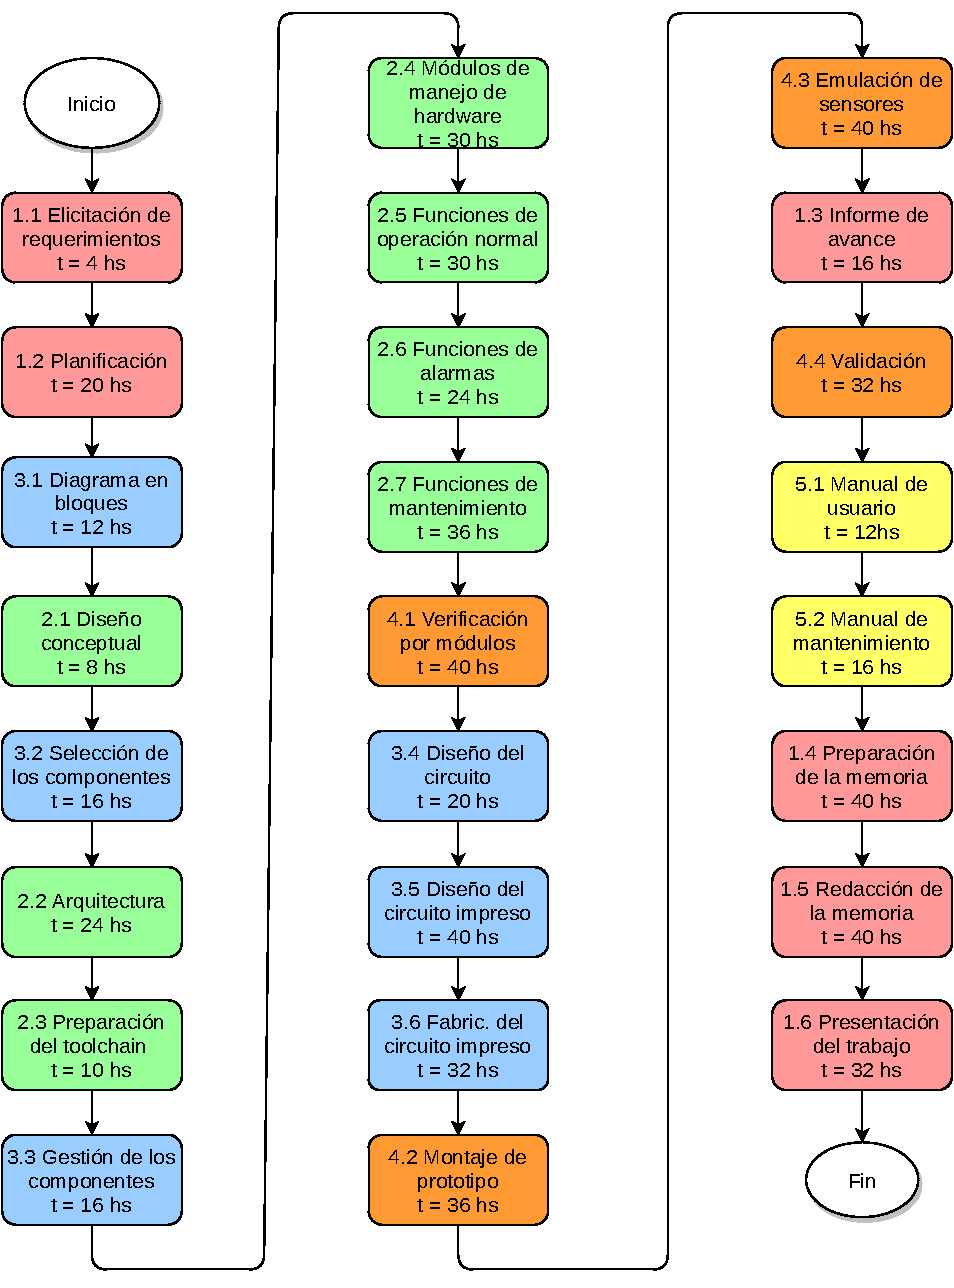
\includegraphics[width=.9\textwidth]{./Figuras/SMTB_AoN.pdf}
\caption{Diagrama en \textit{Activity on Node}}
\label{fig:AoN}
\end{figure}

\section{11. Diagrama de Gantt}
\label{sec:gantt}

Para la elaboración del diagrama de Gantt se consideró una dedicación diaria de 3 horas, de lunes a viernes.

Se utilizó el programa gratuito GanttProject, que solo permite la utilización de días como unidad de tiempo. Por esta razón, se pueden observar algunas diferencias de redondeo en el diagrama.

La planificación se presenta en dos partes para mayor claridad.


\begin{landscape}
\begin{figure}[htpb]
\centering 
\includegraphics
[scale=0.65]
%[width=.99\textwidth]
%[height=.99\textheight]
{./Figuras/SMTB_Gantt_1.png}
\caption{SMTB - Diagrama de Gantt (parte 1 de 2)}
\label{fig:diagGantt}
\end{figure}

\end{landscape}

\begin{landscape}
\begin{figure}[htpb]
\centering 
\includegraphics
[scale=0.5]
%[width=.99\textwidth]
%[height=.99\textheight]
{./Figuras/SMTB_Gantt_2.png}
\caption{SMTB - Diagrama de Gantt (parte 2 de 2)}
\label{fig:diagGantt}
\end{figure}

\end{landscape}


\section{12. Presupuesto detallado del proyecto}
\label{sec:presupuesto}

Para el cálculo del presupuesto se estimo el valor global de los costos indirectos en un 40\% de los costos directos.  

\begin{table}[htpb]
\centering
\begin{tabularx}{\linewidth}{@{}|X|c|r|r|@{}}
\hline
\rowcolor[HTML]{C0C0C0} 
\multicolumn{4}{|c|}{\cellcolor[HTML]{C0C0C0}COSTOS DIRECTOS} \\ \hline
\rowcolor[HTML]{C0C0C0} 
\multicolumn{4}{|c|}{\cellcolor[HTML]{C0C0C0}Materiales} \\ \hline
\rowcolor[HTML]{C0C0C0} 
Descripción &
  \multicolumn{1}{c|}{\cellcolor[HTML]{C0C0C0}Cantidad} &
  \multicolumn{1}{c|}{\cellcolor[HTML]{C0C0C0}Valor unitario} &
  \multicolumn{1}{c|}{\cellcolor[HTML]{C0C0C0}Valor total} \\ \hline
 CIAA-NXP &
  \multicolumn{1}{c|}{2} &
  \multicolumn{1}{c|}{\$ 45.000} &
  \multicolumn{1}{c|}{\$ 90.000} \\ \hline
 Sensor con vaina, conector y cápsula &
  \multicolumn{1}{c|}{36} &
  \multicolumn{1}{c|}{\$ 2.600} &
  \multicolumn{1}{c|}{\$ 93.600} \\ \hline
  
 Gabinete de chapa plegada y máscara &
  \multicolumn{1}{c|}{2} &
  \multicolumn{1}{c|}{\$ 7.500} &
  \multicolumn{1}{c|}{\$ 15.000} \\ \hline
  
  PCB &
  \multicolumn{1}{c|}{1} &
  \multicolumn{1}{c|}{\$ 20.000} &
  \multicolumn{1}{c|}{\$ 20.000} \\ \hline
  
  Display &
  \multicolumn{1}{c|}{2} &
  \multicolumn{1}{c|}{\$ 2.000} &
  \multicolumn{1}{c|}{\$ 4.000} \\ \hline
  
  Componentes adicionales &
  \multicolumn{1}{c|}{1} &
  \multicolumn{1}{c|}{\$ 10.000} &
  \multicolumn{1}{c|}{\$ 10.000} \\ \hline
  

\multicolumn{3}{|c|}{SUBTOTAL} &
  \multicolumn{1}{c|}{\$ 232.600} \\ \hline
  
\multicolumn{4}{|c|}{\cellcolor[HTML]{C0C0C0}Mano de obra} \\ \hline
\rowcolor[HTML]{C0C0C0} 
Descripción &
  \multicolumn{1}{c|}{\cellcolor[HTML]{C0C0C0}Cantidad} &
  \multicolumn{1}{c|}{\cellcolor[HTML]{C0C0C0}Valor unitario} &
  \multicolumn{1}{c|}{\cellcolor[HTML]{C0C0C0}Valor total} \\ \hline
 Ingeniería &
  \multicolumn{1}{c|}{542 hs} &
  \multicolumn{1}{c|}{\$ 1.080} &
  \multicolumn{1}{c|}{\$ 585.360} \\ \hline
  
 Otras tareas &
  \multicolumn{1}{c|}{84 hs} &
  \multicolumn{1}{c|}{\$ 1.080} &
  \multicolumn{1}{c|}{\$ 90.720} \\ \hline
  
\multicolumn{3}{|c|}{SUBTOTAL} &
  \multicolumn{1}{c|}{\$ 676.080} \\ \hline  
  
\rowcolor[HTML]{C0C0C0} 
\multicolumn{4}{|c|}{\cellcolor[HTML]{C0C0C0}COSTOS INDIRECTOS} \\ \hline

\rowcolor[HTML]{C0C0C0} 
\multicolumn{3}{|l|}{Descripción} &
  \multicolumn{1}{c|}{\cellcolor[HTML]{C0C0C0}Valor total} \\ \hline
\multicolumn{3}{|l|}{Estimado global (40\% C.D.)} & \multicolumn{1}{c|}{\$ 363.472 } \\ \hline


\multicolumn{3}{|c|}{SUBTOTAL} &  
  \multicolumn{1}{c|}{\$ 363.472 } \\ \hline
\rowcolor[HTML]{C0C0C0}
\multicolumn{3}{|c|}{TOTAL} &
  \multicolumn{1}{c|}{\$ 1.272.152 } \\ \hline
\end{tabularx}%
\end{table}


\section{13. Gestión de riesgos}
\label{sec:riesgos}
\subsection*{Análisis}

A continuación se presentan los riesgos identificados para el proyecto junto con sus puntuaciones de:
\begin{enumerate}
\renewcommand{\theenumi}{\alph{enumi}} %Letras minúsculas 
	\item severidad (S), del 1 al 10, siendo 10 el grado más alto de importancia para sus consecuencias.
	\item ocurrencia (O), del 1 al 10, siendo 10 el grado más alto de probabilidad de ocurrencia.
	\item nivel de prioridad de riesgo (RPN), que se calcula como el producto de los anteriores y representa un nivel relativo de importancia que permite comparar riesgos. 
\end{enumerate}  


%--------------------------------------------------------------------------------------------------
\textbf{Riesgo 1:} subestimación de los tiempos de ejecución de tareas.
		\begin{itemize}
			\item Severidad (5): severidad media, dado que permite un cierto nivel de corrección.
			\item Ocurrencia (5): probabilidad media, por falta de experiencia en la estimación de tiempos de desarrollo de software. 
		\end{itemize}
%-------------------------------------------------------------------------------------------------
\textbf{Riesgo 2:} imposibilidad de adquirir el convertidor DC/DC de alimentación.
		\begin{itemize}
			\item Severidad (5): severidad media, dado que permite un cierto nivel de corrección.
			\item Ocurrencia (7): probabilidad moderada, dado que no existe proveedor local y no 	es de uso masivo. 
		\end{itemize} 
%-------------------------------------------------------------------------------------------------  
\textbf{Riesgo 3:} dificultad en la importación de los conectores.
		\begin{itemize}
			\item Severidad (7): severidad moderada, dado que son necesarios para la 				compatibilidad con los sensores actuales.
			\item Ocurrencia (5): probabilidad media, dado que no existe proveedor local pero 		existen algunos importadores. 
		\end{itemize} 
%------------------------------------------------------------------------------------------------
\textbf{Riesgo 4:} inestabilidad del master OneWire a implementar por software.
		\begin{itemize}
			\item Severidad (5): severidad media, porque afecta a una funcionalidad principal pero admite corrección por hardware.
			\item Ocurrencia (4): probabilidad media-baja, dado que se conocen implementaciones exitosas en otras plataformas. 
		\end{itemize}   
%-------------------------------------------------------------------------------------------------
\textbf{Riesgo 5:} obtención de confiabilidad baja del producto.
		\begin{itemize}
			\item Severidad (8): severidad moderada-alta, porque afecta a la eficacia total del sistema.
			\item Ocurrencia (3): probabilidad baja, dado que se utiliza tecnología similar al sistema original con confiabilidad aceptada. 
		\end{itemize}   
%-------------------------------------------------------------------------------------------------	
\textbf{Riesgo 6:} pérdida de las herramientas de trabajo.
		\begin{itemize}
			\item Severidad (9): severidad alta, porque se posee un solo equipo dedicado al proyecto.
			\item Ocurrencia (3): probabilidad baja, dado que el equipo solo se transporta excepcionalmente.
		\end{itemize}   
%-------------------------------------------------------------------------------------------------
\textbf{Riesgo 7:} pérdida de los avances realizados en el desarrollo.
		\begin{itemize}
			\item Severidad (8): severidad moderada-alta, porque dependiendo del momento de la pérdida puede penalizar fuertemente el cronograma de trabajo.
			\item Ocurrencia (1): probabilidad muy baja, dado que se almacenará el trabajo en un repositorio en linea y con control de versiones.
		\end{itemize}   
%-------------------------------------------------------------------------------------------------
\textbf{Riesgo 8:} cambio significativo de los costos presupuestados de materiales.
		\begin{itemize}
			\item Severidad (6): severidad media-moderada, porque el peso presupuestario de los materiales es relativamente bajo.
			\item Ocurrencia (5): probabilidad media, dadas las proyecciones económicas disponibles.
		\end{itemize}   
%------------------------------------------------------------------------------------------------

\subsection*{Plan de mitigación}

Se adopta el criterio de tomar acciones de mitigación para aquellos riesgos que superen los 25 puntos RPN.Ver cuadro 1.
 
\begin{table}[htpb]
\centering
\begin{tabularx}{\linewidth}{@{}|c|X|c|c|c|c|c|c|@{}}
\hline
\rowcolor[HTML]{C0C0C1} 
N & Riesgo & S & O & RPN & S* & O* & RPN* \\ \hline
1& Subestimación de los tiempos de ejecución de tareas& 5 & 5 & 25 &    &    &      \\ \hline
2& Imposibilidad de adquirir el convertidor DC/DC de alimentación& 5& 7&\cellcolor[rgb]{1,.4,0} 35& 5& 2& \cellcolor[rgb]{0,0.7,0}10 \\ \hline
3& Dificultad en la importación de los conectores& 7& 5&\cellcolor[rgb]{1,.4,0} 35& 7& 1& \cellcolor[rgb]{0,0.7,0}7      \\ \hline
4& Inestabilidad del master OneWire a implementar por software& 5& 4& 20&    &    &      \\ \hline
5& Obtención de confiabilidad baja del producto& 8& 3& 24&    &    &      \\ \hline
6& Pérdida de las herramientas de trabajo& 9& 3&\cellcolor[rgb]{1,.4,0} 27& 3& 3&\cellcolor[rgb]{0,0.7,0} 9  \\ \hline
7& Pérdida de los avances realizados en el desarrollo& 8& 1& 8&    &    &      \\ \hline
8& Cambio significativo de los costos presupuestados de materiales& 6& 5&\cellcolor[rgb]{1,.4,0} 30& 5& 4& \cellcolor[rgb]{0,0.7,0} 20   \\ \hline
\end{tabularx}%
\caption{Comparación de riesgos.}
\end{table}

Nota: los valores marcados con (*) en la tabla corresponden luego de haber aplicado la mitigación.

\textbf{Riesgo 2:} se tendrá alistado un diseño alternativo de convertidor con componentes discretos de fácil consecución, para usar solo en prototipos.
  \begin{itemize}
		\item Severidad (5): sin cambios.
		\item Ocurrencia (2): probabilidad baja, se mejoran las posibilidades de adquisición. 
		\end{itemize} 
\textbf{Riesgo 3:} se convendrá con el cliente la provisión de conectores reutilizables, para usar solo en prototipos.
  \begin{itemize}
		\item Severidad (7): sin cambios.
		\item Ocurrencia (1): probabilidad muy baja, se asegura la disponibilidad. 
		\end{itemize}
 
\textbf{Riesgo 6:} se contratará un seguro que cubra la pérdida de la computadora laptop de trabajo.
  \begin{itemize}
		\item Severidad (3): se asegura una alternativa en un tiempo relativamente corto ante la pérdida del equipo.
		\item Ocurrencia (3): sin cambios.
		\end{itemize}
		
\textbf{Riesgo 8:} se priorizarán las tareas de selección y adquisición de materiales, y se agrega a los supuestos del proyecto, de manera de concientizar al cliente de este riesgo.
  \begin{itemize}
		\item Severidad (5): se transfiere parte del impacto al cliente al participarlo del riesgo.
		\item Ocurrencia (4): se minimizan los tiempos hasta la adquisición y por ende la probabilidad de ocurrencia. 
		\end{itemize}

\section{14. Gestión de la calidad}
\label{sec:calidad}
A continuación se detallan los procedimientos de verificación y validación para cada requerimiento: 
% Req 1.1----------------------------------------------------------------------------------
\begin{itemize} 
\item Requerimiento 1.1.: el sistema debe conservar el factor de forma de la unidades, alimentación eléctrica, conectores y cables del sistema original reemplazado.
\begin{itemize}
	\item Verificación: finalizada la etapa de diseño se verificarán las medidas mecánicas y características eléctricas y se plasmarán en un informe de compatibilidad. 
	\item Validación: para realizar las pruebas funcionales el sistema se armará completamente, lo que confirmará la compatibilidad. 
\end{itemize}
% Req 1.2----------------------------------------------------------------------------------
\item Requerimiento 1.2.: los sensores deberán ser intercambiables con los del sistema reemplazado.
\begin{itemize}
	\item Verificación: se realizará el análisis de un sensor actual con el fin de identificarlo y relevar las características mecánicas de su implementación. 
	\item Validación: se realizarán pruebas funcionales con sensores actuales instalados.
\end{itemize}
% Req 1.3----------------------------------------------------------------------------------
\item Requerimiento 1.3.: la comunicación entre UCIs no podrá utilizar más de 4 conductores (6 existentes, 2 reservados para alimentación de la UCI\#2).
\begin{itemize}
	\item Verificación: se analizará al momento de la determinación del tipo de comunicación a utilizar entre UCIs.
	\item Validación: se incluirá en la prueba funcional de comunicación. 
\end{itemize}
% Req 1.4----------------------------------------------------------------------------------
\item Requerimiento 1.4.: los modelos de UCI podrán ser intercambiables, incluyendo un medio de selección de la posición en que se instalan. Se debe incluir en el software un algoritmo para resolución de conflictos por selección errónea. 
\begin{itemize}
	\item Verificación: se realizará una prueba de banco donde se armará todo el sistema fuera de la locomotora (mock up) e incluirá este item.
	\item Validación: Se incluirá en las pruebas funcionales el intercambio de las UCI y el seteo erróneo ex profeso para validar la resolución del conflicto. 
\end{itemize}
% Req 2.1----------------------------------------------------------------------------------
\item Requerimiento 2.1.: el sistema deberá gestionar un bus al que se conectan 36 sensores de temperatura tipo DS18B20 (bus\#1).  
\begin{itemize}
	\item Verificación: se incluirá en las pruebas de mock up.  
	\item Validación: se incluirá en las pruebas de funcionales.
\end{itemize}
% Req 2.1----------------------------------------------------------------------------------
\item Requerimiento 2.2.: deberá registrar de manera no volátil (EEPROM) la correspondencia del ID de sensor con la ubicación en que se encuentra, en ambas UCI. 
\begin{itemize}
	\item Verificación: se realizarán pruebas de ubicación calentando individualmente los sensores del mock up. 
	\item Validación: se realizarán pruebas de ubicación calentando individualmente los sensores de la locomotora. 
\end{itemize}
% Req 2.1----------------------------------------------------------------------------------
\item Requerimiento 2.3.: el sistema deberá gestionar un bus al que se conectará un solo sensor a la vez, para permitir su alta individual en el registro ROM (bus\#2).  
\begin{itemize}
	\item Verificación: se realizará pruebas de alta en el mock up. 
	\item Validación: se realizará pruebas de alta en la locomotora.
\end{itemize}
% Req 2.1----------------------------------------------------------------------------------
\item Requerimiento 2.4.: se deberá permitir la operación degradada (sensores fuera de 				servicio y/o UCI\#2 fuera de servicio). 
\begin{itemize}
	\item Verificación: se realizarán pruebas desconectando sensores o UCI, según corresponda, en el mock up.
	\item Validación: se realizarán pruebas desconectando sensores o UCI, según corresponda, en la locomotora.
\end{itemize}
% Req 2.1----------------------------------------------------------------------------------
\item Requerimiento 2.5.: el sistema deberá evaluar la condición de alarma según el algoritmo a definir. 
\begin{itemize}
	\item Verificación: se realizarán pruebas de alarma emulando sensores en el mock up. 
	\item Validación: se realizarán pruebas calentando sensores en la locomotora.
\end{itemize}
% Req 2.1----------------------------------------------------------------------------------
\item Requerimiento 2.6.: la condición de alarma deberá ser informada por el sistema de	manera visual y sonora. 
\begin{itemize}
	\item Verificación: se incluirán en las pruebas de verificación del requerimiento 2.5.
	\item Validación: se incluirán en las pruebas de validación del requerimiento 2.5.
\end{itemize}
% Req 2.1----------------------------------------------------------------------------------
\item Requerimiento 2.7.: la alarma sonora tendrá la posibilidad de ser silenciada, 				volviendo a activarse cíclicamente, en tanto la condición de alarma continúe. 
\begin{itemize}
	\item Verificación: se incluirá en las pruebas de verificación del requerimiento 2.5.
	\item Validación: se incluirá en las pruebas de validación del requerimiento 2.5.
\end{itemize}
% Req 2.1----------------------------------------------------------------------------------
\item Requerimiento 2.8.: la alarma visual no podrá ser desactivada, en tanto la condición de alarma continúe.  
\begin{itemize}
	\item Verificación: se incluirá en las pruebas de verificación del requerimiento 2.5.
	\item Validación: se incluirá en las pruebas de validación del requerimiento 2.5.
\end{itemize}
% Req 2.1----------------------------------------------------------------------------------
\item Requerimiento 2.9.: las unidades UCI deberán comunicarse con los buses de sensores a través del protocolo OneWire. 
\begin{itemize}
	\item Verificación: se realizará prueba individual de módulo de software de protocolo OneWire.
	\item Validación: está incluido en las pruebas de funcionamiento.
\end{itemize}
% Req 2.1----------------------------------------------------------------------------------
\item Requerimiento 2.10.: cada unidad UCI deberá contar con un display LCD de tipo gráfico o texto. 
\begin{itemize}
	\item Verificación: incluido en las pruebas individuales de módulo de software HMI. 
	\item Validación: incluido en las pruebas funcionales.
\end{itemize}
% Req 2.1----------------------------------------------------------------------------------
\item Requerimiento 2.11.: cada unidad UCI deberá contar una matriz LED de 6 x 6, que se utilizará para mostrar ubicaciones correspondiendo cada fila al número de eje y cada columna al número de sensor. 
\begin{itemize}
	\item Verificación: incluido en las pruebas individuales de módulo de software HMI. 
	\item Validación:  incluido en las pruebas funcionales.
\end{itemize}
% Req 2.1----------------------------------------------------------------------------------
\item Requerimiento 2.12.: cada unidad UCI deberá contar con pulsadores, en número no menor a cuatro, para permitir el ingreso de opciones de menú o selección de ubicaciones por parte del usuario. 
\begin{itemize}
	\item Verificación: se incluirá en las pruebas individuales de módulo de software HMI. 
	\item Validación: se incluirá en las pruebas funcionales.
\end{itemize}
% Req 2.1----------------------------------------------------------------------------------
\item Requerimiento 2.13.:  Cada unidad UCI deberá contar con un pulsador (aparte de los requeridos en el item anterior para permitir el reset total del sistema. 
\begin{itemize}
	\item Verificación: se verificará en la selección de hardware. 
	\item Validación: incluido en las pruebas funcionales.
\end{itemize}
% Req 2.1----------------------------------------------------------------------------------
\item Requerimiento 2.14.: El tiempo entre actualización de un dato de temperatura en particular no deberá exceder los 60 segundos.
\begin{itemize}
	\item Verificación: se incluirá en el software una señalización para permitir la medición (mock up).
	\item Validación: se mostrará la prueba de verificación al cliente, dada la imposibilidad de validar en funcionamiento normal.
\end{itemize}
% Req 2.1----------------------------------------------------------------------------------
\item Requerimiento 2.15.: Se deberá contar con una función de registro de alarmas (datalogging).  
\begin{itemize}
	\item Verificación: se incluirá en las pruebas de verificación del requerimiento 2.5.
	\item Validación: se incluirá en las pruebas de validación del requerimiento 2.5. 
\end{itemize}
% Req 2.1----------------------------------------------------------------------------------
\item Requerimiento 3.1.: El sistema deberá mostrar los mensajes de estados y menúes en el display LCD, mediante texto.  
\begin{itemize}
	\item Verificación: se incluirá en las pruebas individuales de módulo de software HMI. 
	\item Validación: se incluirá en las pruebas funcionales.
\end{itemize}
% Req 2.1----------------------------------------------------------------------------------
\item Requerimiento 3.2.: El sistema deberá mostrar información referente al estado del sensor mediante la matriz LED. Para ello, encenderá de modo fijo el LED correspondiente a la temperatura mostrada en display y de modo intermitente el que corresponda a un sensor fuera de servicio. 
\begin{itemize}
	\item Verificación: se incluirá en las pruebas individuales de módulo de software HMI. 
	\item Validación: se incluirá en las pruebas funcionales.
\end{itemize}
% Req 2.1----------------------------------------------------------------------------------
\item Requerimiento 3.3.: El sistema no se limitará a mostrar las ubicaciones solo en la matriz LED. Lo hará además en el display LCD, mediante texto.  
\begin{itemize}
	\item Verificación: se incluirá en las pruebas individuales de módulo de software HMI. 
	\item Validación: se incluirá en las pruebas funcionales.
\end{itemize}
% Req 2.1----------------------------------------------------------------------------------
\item Requerimiento 4.1.: El sistema deberá evaluar su condición de funcionamiento e informar su estado. Como mínimo deberá incluirse:
\begin{enumerate}
\renewcommand{\theenumi}{\alph{enumi}} %Letras minúsculas 
	\item comunicación entre UCIs
	\item comunicación con sensores
	\item existencia y consistencia de registros ROM
	\item alta de sensores en ROM).
\end{enumerate}  
\begin{itemize}
	\item Verificación: se incluirá en las pruebas individuales de módulos de software. 
	\item Validación: se incluirá en las pruebas funcionales.
\end{itemize}
% Req 2.1----------------------------------------------------------------------------------
\item Requerimiento 4.2.: El autochequeo se realizará automáticamente al iniciar el sistema y a requerimiento del usuario.  
\begin{itemize}
	\item Verificación: se incluirá en las pruebas individuales de módulos de software. 
	\item Validación: se incluirá en las pruebas funcionales. 
\end{itemize}
% Req 2.1----------------------------------------------------------------------------------
\item Requerimiento 4.3.: Se utilizarán las memorias ROM de ambas UCI como respaldo de la otra, para facilitar el alta de todos los sensores ante el cambio de una UCI. 
\begin{itemize}
	\item Verificación: se incluirá en las pruebas individuales de módulos de software. 
	\item Validación: se incluirá en las pruebas funcionales. 
\end{itemize}
% Req 2.1----------------------------------------------------------------------------------
\item Requerimiento 4.4.: Se proveerá soporte para un procedimiento de alta de sensor (registro de ID y su ubicación).  
\begin{itemize}
	\item Verificación: 
\end{itemize}
% Req 2.1----------------------------------------------------------------------------------
\item Requerimiento 4.5.: El alta de sensor podrá realizarse de manera individual por el bus\#2; o de manera secuencial para todos los sensores instalados por el bus\#1 (bus normal de trabajo de los sensores). 
\begin{itemize}
	\item Verificación: se incluirá en las pruebas individuales de módulos de software. 
	\item Validación: se incluirá en las pruebas funcionales. 
\end{itemize}
% Req 2.1----------------------------------------------------------------------------------
\item Requerimiento 5.1.: El sistema se proveerá con su manual de operación. 
\begin{itemize}
	\item Verificación: se verificará la inclusión en la planificación.
	\item Validación: esta incluido en los entregables de proyecto. 
\end{itemize}
% Req 2.1----------------------------------------------------------------------------------
\item Requerimiento 5.2.: El sistema se proveerá con su manual de mantenimiento. 
\begin{itemize}
	\item Verificación: se verificará la inclusión en la planificación.
	\item Validación: esta incluido en los entregables de proyecto. 
\end{itemize}

\end{itemize}

\section{15. Procesos de cierre}    
\label{sec:cierre}

Sobre la finalización del proyecto se ejecutará la etapa de su cierre que consistirá de los siguientes procesos:  

\begin{itemize}
	\item Análisis de las pautas de trabajo:
	\begin{itemize}
		\item Persona a cargo: Ing. Hernán Gomez Molino.
		\item Procedimiento: se analizará el cumplimiento de la planificación original del proyecto en cuanto a fechas, recursos asignados y requerimientos. 
		\end{itemize}
	\item Relevamiento de las técnicas y procedimientos utilizados:
	\begin{itemize}
		\item Persona a cargo: Ing. Hernán Gomez Molino. 
		\item Procedimiento: se evaluarán las técnicas y procedimientos aplicados, en cuanto a su utilidad. También se analizarán los imprevistos surgidos y las soluciones implementadas.
	\end{itemize}
	\item Acto de cierre:
	\begin{itemize}
		\item Persona a cargo: Ing. Hernán Gomez Molino. 
		\item Procedimiento: El responsable del proyecto estará a cargo de realizar un acto de cierre, donde se agradecerá a todos los involucrados en el proyecto, miembros del jurado, docentes y autoridades de la CESE. 
	\end{itemize}
\end{itemize}

\end{document}
